\section{grundlegende Antennentheorie}
\label{sec:basic-ant}
\subsection{Antennenfeldzonen}
Das von einer Antenne abgestrahlte Feld lässt sich in 3 verschiedene Regionen einteilen: das Nahfeld, das Übergangsfeld (Fresnel-Region) und das Fernfeld (Fraunhofer-Region)\cite{antenna_field_zones}.\\

Je nach Literatur erfolgt der Übergang zwischen den Feldzonen fließend. Eine Möglichkeit die Zonen einzuteilen ist in der nachfolgenden Tabelle einzusehen.

\begin{center}
	\begin{tabular}[h]{|c|c|c| p{"5"cm}}
		\hline
		Nahfeld & Übergangsfeld & Fernfeld\\
		\hline
		r $<$ 0.2 $\lambda$ & 0.2 $\leq$ r $\leq$ 4$\lambda$ & r $>$ 0.4$\lambda$\\
		\hline
	\end{tabular}
\end{center}

Das Nahfeld ist darin besonders, dass das elektrische und magnetische Feld mit unterschiedlichen Faktoren in Abhängigkeit der Entfernung abnehmen. Im Übergangsfeld nehmen das elektrische und magnetische Feld zwar mit dem gleichen Faktor ab, jedoch unterscheiden Sie sich noch in der Phase und Amplitude.\\

Im Gegensatz zum reaktiven Nahfeld wird beim Fernfeld Wirkleistung abgestrahlt. Hierbei sind die elektrische und magnetische Komponente der Welle in Phase und nehmen im gleichen Maß ab.\\

Da unsere Diplomarbeit einen Fokus auf die Satellitentechnik hat, ist für dieses Dokument nur das Fernfeld relevant. 

\subsection{Polarisation}
\label{subsec:pol}
Die Polarisationsart wird von der Ausrichtung des Vektors der elektrischen Feldstärke bestimmt. Es lässt sich zwischen drei verschiedenen Arten der Polarisation unterscheiden.\\


\begin{enumerate}
	\item Lineare Polarisation
	\begin{enumerate}
		\item horizontale Polarisation
		Eine horizontale Polarisation liegt vor, wenn die Feldlinien parallel zum Boden verlaufen.
		\item vertikale Polarisation
		Die vertikale Polarisation entsteht, wenn die elektrischen Feldlinien senkrecht zum Erdboden stehen.
	\end{enumerate}
	\item Zirkulare Polarisation
	Der Betrag des elektrischen Feldstärkevektors ist konstant. Der Feldstärkevektor rotiert in einer Spirale um den in Ausbreitungsrichtung weisenden Vektor. Ein Spiralumlauf ist nach der Wellenlänge $\lambda$ vollendet.
	\item Elliptische Polarisation
	Betrag sowie Richtung des elektrischen Feldstärkevektors ändern sich laufend. Bei der Rotation beschreibt der Vektor eine Ellipse.
\end{enumerate}

Für diese Diplomarbeit liegt der Fokus auf der zirkularen Polarisation. Diese ist in der Satellitenkommunikationstechnik äußerst beliebt, da sie Immunität vor den störenden Effekten in der Ionosphäre, spezieller der Faraday Rotation, bieten.

Die Faraday Rotation ist ein Effekt, welcher elektromagnetische Strahlung $"$rotiert$"$. Dies ist problematisch für linear polarisierte Strahlung, aber keines für zirkular polarisierte. Da die zirkulare Polarisation schon von ihrer Natur her eine rotierende elektromagnetische Welle mit sich bringt, ändert sich für diese nichts wenn sie in die Ionosphäre eintritt \cite{takashi_encyclopedia_2003}.

\subsection{Kenngrößen einer Antenne}

\subsubsection{Antennengewinn}
Als Antennengewinn wird die $"$bündelnde$"$ Eigenschaft einer gerichteten Antenne im Vergleich zu einer Bezugsantenne bezeichnet. Hierbei ist die Vergleichsantenne meist ein Kugelstrahler.\\

Der Gewinn der Antenne berechnet sich mit dem Verhältnis der maximalen Empfangsleistung der gerichteten Antenne zu der des Kugelstrahlers. Wird als Bezugsantenne der Kugelstrahler verwendet, so wird die Empfangsleistung mit dem Index 'i' versehen um dies zu kennzeichnen.

\begin{equation}
	G=\frac{P_{max}}{P_{i}}
\end{equation}

\subsubsection{Welligkeit}
Die Welligkeit oder das Stehwellenverhältnis (SWR) gibt Aufschluss über die Spannungsverteilung auf der Speiseleitung und ist ein Maß für die Qualität der Anpassung. Sie beschreibt, wie groß der Anteil der reflektierten Wellen ist. Je schlechter die Anpassung, desto größer der Anteil der Wellen, welche reflektiert werden und desto größer das SWR.\\

\begin{equation}
	SWR=\frac{U_{max}}{U_{min}}=\frac{I_{max}}{I_{min}}=\frac{1+\lvert \rho \lvert}{1-\lvert \rho \lvert}
\end{equation}

Wobei $\rho$ der Reflexionsfaktor ist. Der Reflexionsfaktor kann auch der Streumatrix entnommen werden, welche


\subsubsection{effektive Antennenfläche}
Die effektive Antennenfläche ist das Verhältnis zwischen der Leistung welche von der Antenne aufgenommen und an eine angeschlossene Last abgegeben wird zu der Leistung welche die eingehende Welle liefert. Sie wird in $m^2$ angegeben.

\subsubsection{Halbwertsbreite}
Zur Bestimmung der Halbwertsbreite ist die Hauptkeule des Abstrahldiagramms einer Antenne von Relevanz. Die Halbwertsbreite ist hierbei der Öffnungswinkel, der geformt wird, wenn die Amplitude der Hauptkeule auf 50 Prozent oder um 3dB abgesunken ist.

\subsubsection{Eingangsimpedanz}
Die Eingangsimpedanz einer Antenne ist eine wichtige Größe in der Antennentechnik. Dies liegt daran, dass die Antenne meist auf ein Koaxialkabel mit einem Wellenwiderstand von 50$\Omega$ angepasst werden muss. Dies kann durch verschiedene Anpassungstechniken erreicht werden, wie z.B. ein LC-Anpassungsnetzwerk oder Übertragungsleitungen. 

\subsubsection{S11 Parameter}
Der S11 Parameter beschreibt, wie viel eines Signals an dem Tor eines Vierpols reflektiert wird. Hierbei wird das Verhältnis zwischen hinlaufender Welle und rücklaufender Welle aufgestellt. Mithilfe dieses Parameters kann auf die Qualität der Impedanzanpassung geschlossen werden. Je niedriger der Wert, desto besser die Anpassung. Der S11 Parameter wird üblicherweise in dB angegeben MISSING REFERENCE.

\subsection{Richtcharakteristik und Richtdiagramm}
Die Richtcharakteristik beschreibt das Abstrahlverhalten einer Antenne. Hierbei wird die unter einem bestimmten Winkel ($\theta$, $\phi$) auftretende Feldstärke auf einen Maximalwert bezogen.

\begin{equation}
	C(\theta, \phi)=\frac{E(\theta, \phi)}{E_{max}}
\end{equation}

Wobei $\theta$ der Elevationswinkel (vertikal Winkel) und $\phi$ den Azimutwinkel (horizontaler Winkel) repräsentiert.

\begin{figure}[H]
	\centering
	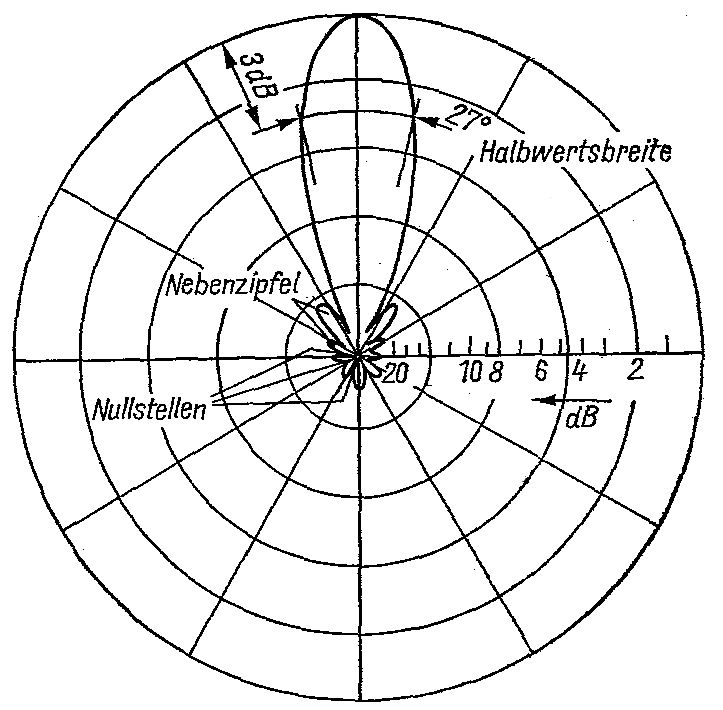
\includegraphics[width=\textwidth]{../ref/Richtdiagramm_Beispiel}
	\caption{Richtdiagramm einer stark bündelnden Antenne}
	\label{fig:Richtdiagramm Beispiel}
\end{figure}

Hierbei ist zu bemerken dass in Abbildung \ref{fig:Richtdiagramm Beispiel} entgegen der üblichen Konvention das Richtdiagramm aus dem Verhältnis zwischen Strahlungsleistungsdichte und ihrem Maximalwert ergibt. Es ist gebräuchlich, das Diagramm auf den Maximalwert zu normieren, sodass sich bei der maximalen Feldstärke 0 dB Dämpfung ergeben.\\

Der größte Teil der Leistung ist naheliegend in der Hauptkeule zu finden, während es nötig ist die Neben-und Rückwärtskeulen möglichst klein zu halten, um unnötige Abstrahlung in die Umgebung zu vermeiden. Die Halbwertsbreite der Hauptkeule ist der Wert ab dem die Leistungsdichte auf die Hälfte abgesunken ist.\\

Eine weitere wichtige Kenngröße bei Richtantennen ist das Vor-Rückwärtsverhältnis. Dies ist die Fähigkeit einer Richtantenne, Strahlung aus anderen Richtungen als der Hauptstrahlrichtung zu unterdrücken.

\subsection{Einfluss der Erde auf das Richtdiagramm}
Wird das Strahlungsdiagramm einer Antenne über dem Boden mit dem einer Antenne im Freiraum verglichen, lassen sich große Unterschiede erkennen. Der Boden dient als Reflektor wobei seine Reflexionseigenschaften von der Dielektrizitätskonstante sowie der Leitfähigkeit bestimmt werden.\\

Für die Reflexion elektromagnetischer Wellen am Erdboden trifft das Reflexionsgesetz zu, das bedeutet, dass der Einfallswinkel gleich dem Ausfallswinkel ist. Hierbei kann es zu Überlagerungen zwischen den reflektierten und nicht reflektierten Wellen kommen und somit können destruktive und konstruktive Interferenzen entstehen.\\

Die Polarisierung der verwendeten Antenne spielt eine entscheidende Rolle bei der Reflexion. Bei einer vertikal polarisierten Antenne ist der Stromverlauf von Spiegelbild und Original gleichphasig. Bei einer horizontal polarisierten Antenne hingegen ist der Stromverlauf zwischen Reflexion und Original gegenphasig.\\

Der Abstand vom Boden spielt ebenfalls eine kritische Rolle und hat großen Einfluss auf das resultierende Richtdiagramm der Antenne. Wird beispielsweise ein Dipol $\frac{\lambda}{2}$ vom Boden entfernt aufgestellt, so verändert sich sein Richtdiagramm so sehr, dass aus der omnidirektionalen Antenne ein Strahler mit zwei Strahlungskeulen wird. 


\subsection{Baluns}
Um Baluns zu verstehen muss vorerst der Unterschied zwischen symmetrischen und unsymmetrischen Leitungen verstanden werden. 

Eine unsymmetrische Leitung besteht aus einem Hauptleiter und einer Masseleitung, welche oft als Schild vor Störstrahlung verwendet wird. Jedoch ist das Kabel nicht nur gegen externe Strahlung geschützt, das Kabel selbst strahlt ebenfalls nicht. Das wohl bekannteste Beispiel hierfür sind Koaxialkabel. Eine symmetrische Leitung hingegen besitzt keinen Mantel und kann strahlen SOURCE. Ein Beispiel für eine symmetrische Antenne ist eine QHA (Quadrifilare Helixantenne). Da symmetrische Antennen meist durch unsymmetrische Kabel (Koaxialkabel) betrieben werden, entsteht ein Problem. Es können Mantelwellen auf dem Koaxialkabel auftreten, was dazu führt, dass das Kabel strahlt. Außerdem wird dadurch das Abstrahlverhalten der Antenne beeinflusst, was die Funktion der Antenne beeinträchtigt. Um diese Nebeneffekte zu kompensieren werden Baluns eingesetzt.

\subsubsection{Mantelwellensperre}
Eine Mantelwellensperre ist wie folgt aufgebaut:


Sie unterdrückt Mantelwellen, welche negative Auswirkungen auf das Abstrahlverhalten der Antenne haben. Der Nachteil ist, dass sie schwach gegen statische Entladungen ist, da keine galvanische Isolierung existiert, wie beim Transformator. Sie ist für Anwendungen geeignet, in denen galvanische Isolierung nicht von allzu großer Relevanz ist.

\subsubsection{Transformator}
Der Transformator bietet mehrere Vorteile. Zum einen isoliert dieses Bauteil die Antenne galvanisch vom Rest des Netzwerkes, und zum anderen kann ein beliebiges Übersetzungsverhältnis gewählt werden. Der Transformator sollte gewählt werden, wenn ein guter Schutz gegen statische Entladungen gefordert ist. Allerdings ist anzumerken, dass der Transformator keinen Schutz gegen Mantelwellen bietet.

